\documentclass{article}
\usepackage{geometry} \geometry{margin=1in}
\usepackage{parskip}
\usepackage{ragged2e}
\usepackage{float}       % Required for [H]
\usepackage{tcolorbox}
\usepackage{amsmath, amssymb}
\usepackage{hyperref}     % Fixes "URL" errors
\usepackage{adjustbox}    % CRITICAL: Allows us to shrink huge diagrams
\usepackage{listings}     % For code blocks

% EXTENDED TIKZ LIBRARIES (Fixes "unknown library" errors)
\usepackage{tikz} 
\usetikzlibrary{shapes, arrows.meta, positioning, shadows, calc, fit, backgrounds, decorations.pathreplacing}

% GLOBAL STYLES
\tikzset{
    block/.style={rectangle, draw, thick, rounded corners, fill=blue!5, align=center, minimum height=2em},
    arrow/.style={thick, ->, >=stealth},
    decision/.style={diamond, draw, fill=green!10, align=center, aspect=2},
    cloud/.style={draw, ellipse, fill=red!10, node distance=3cm, minimum height=2em}
}
\raggedbottom

\begin{document}

% --- START OF CHUNK 1 ---

\section{Cybersecurity Fundamentals and Penetration Testing}

\subsection{Essential Protocols and Ports}

Understanding network protocols and the ports they utilize is fundamental to cybersecurity.  Ports are virtual pathways that allow communication between different applications and services on a network.  Each service typically listens on a specific port number.  Knowing these standard port assignments is crucial for network security analysis, intrusion detection, and firewall configuration. For example, **FTP** (File Transfer Protocol) commonly uses ports 20 and 21 for data and control connections, respectively. **SSH** (Secure Shell), a secure remote access protocol, operates on port 22.  **HTTP** (Hypertext Transfer Protocol) uses port 80 for unencrypted web traffic, while its secure counterpart, **HTTPS** (Hypertext Transfer Protocol Secure), uses port 443.  Other important protocols include **SMTP** (Simple Mail Transfer Protocol) on port 25 for email sending, **DNS** (Domain Name System) on port 53 for domain name resolution, and **RDP** (Remote Desktop Protocol) on port 3389 for remote access to graphical user interfaces.  Security professionals must be aware of these standard ports to identify potentially malicious traffic or vulnerabilities.

\subsection{Types of Hackers}

The term "hacker" often carries negative connotations, but it encompasses a wide range of individuals with varying motivations and skill levels.  A **white hat hacker**, often referred to as a **penetration tester**, uses their skills ethically and legally. They are authorized to probe systems for vulnerabilities with the explicit permission of the system owners.  Their goal is to identify weaknesses before malicious actors can exploit them. In contrast, a **black hat hacker** engages in illegal and unethical activities, gaining unauthorized access to systems with the intent to cause harm, steal data, or disrupt services. Black hat hackers are sometimes referred to as **crackers**.  Finally, a **gray hat hacker** occupies a middle ground. They may engage in activities that are technically illegal, such as probing systems without explicit permission, but their intent is not typically malicious. They might disclose vulnerabilities to the system owner, sometimes demanding a reward.

\subsection{Penetration Testing (PenTesting)}

**Penetration testing**, also known as **ethical hacking**, is a simulated cyberattack against a computer system to evaluate its security.  It is an **authorized** attempt to discover vulnerabilities that a malicious attacker could exploit.  Penetration testers are typically employed by companies or security firms and follow a structured methodology to identify weaknesses in a target's security posture.  The process involves several stages, from initial reconnaissance to exploitation and reporting.  The ultimate goal is to provide the organization with a detailed report outlining the identified vulnerabilities, their potential impact, and recommendations for remediation.  This allows the organization to proactively address security gaps and reduce its risk of a successful attack.

\subsection{Penetration Testing Stages}

The penetration testing process is not random; it follows a series of well-defined stages.  The initial stage, **Planning and Reconnaissance**, involves defining the scope of the test and gathering intelligence about the target system. This includes identifying network infrastructure, operating systems, and potential vulnerabilities.  Next, **Scanning** utilizes various tools to understand how the target responds to different types of probes and identify open ports and services.  **Gaining Access** involves exploiting identified vulnerabilities to gain unauthorized access to the system.  This may involve techniques such as SQL injection, cross-site scripting, or exploiting weak passwords.  Once access is gained, **Maintaining Access** focuses on establishing a persistent presence on the system, often by installing backdoors or escalating privileges.  Finally, **Analysis and WAF Configuration** involves analyzing the results of the penetration test and providing recommendations for remediation. This may include configuring a **Web Application Firewall (WAF)** to protect against future attacks.

\begin{figure}[H]
    \centering
    \begin{adjustbox}{max width=\textwidth}
        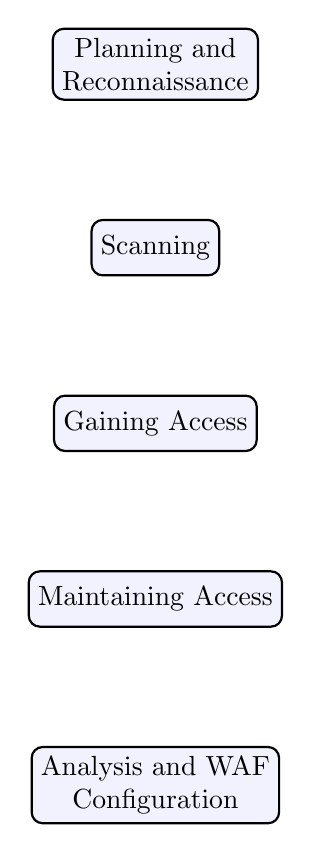
\begin{tikzpicture}[node distance=1.5cm, auto]
            \node[block, align=center] (plan) {Planning and\\Reconnaissance};
            \node[block, align=center, below=of plan] (scan) {Scanning};
            \node[block, align=center, below=of scan] (gain) {Gaining Access};
            \node[block, align=center, below=of gain] (maintain) {Maintaining Access};
            \node[block, align=center, below=of maintain] (analyze) {Analysis and WAF\\Configuration};

            \path[arrow] (plan) -- (scan);
            \path[arrow] (scan) -- (gain);
            \path[arrow] (gain) -- (maintain);
            \path[arrow] (maintain) -- (analyze);
        \end{tikzpicture}
    \end{adjustbox}
    \caption{Penetration Testing Stages - Simplified}
\end{figure}

A more detailed view of the penetration testing stages reveals a cyclical process of information gathering, enumeration, vulnerability identification, and exploitation.  **Information gathering** involves scoping the target and understanding the customer's business. **Enumeration** focuses on discovering open ports, services, and web application pages. **Vulnerability identification** utilizes automated scans and manual techniques to uncover weaknesses. **Attack surface analysis** determines potential attack vectors and develops an attack plan.  **Pivot** involves identifying new targets based on information gained during the process. **Penetration and exploitation** focuses on exploiting vulnerabilities, starting with the easiest targets. Finally, **Privilege escalation** aims to elevate permissions and gain further access to the system.

\begin{figure}[H]
    \centering
    \begin{adjustbox}{max width=\textwidth}
        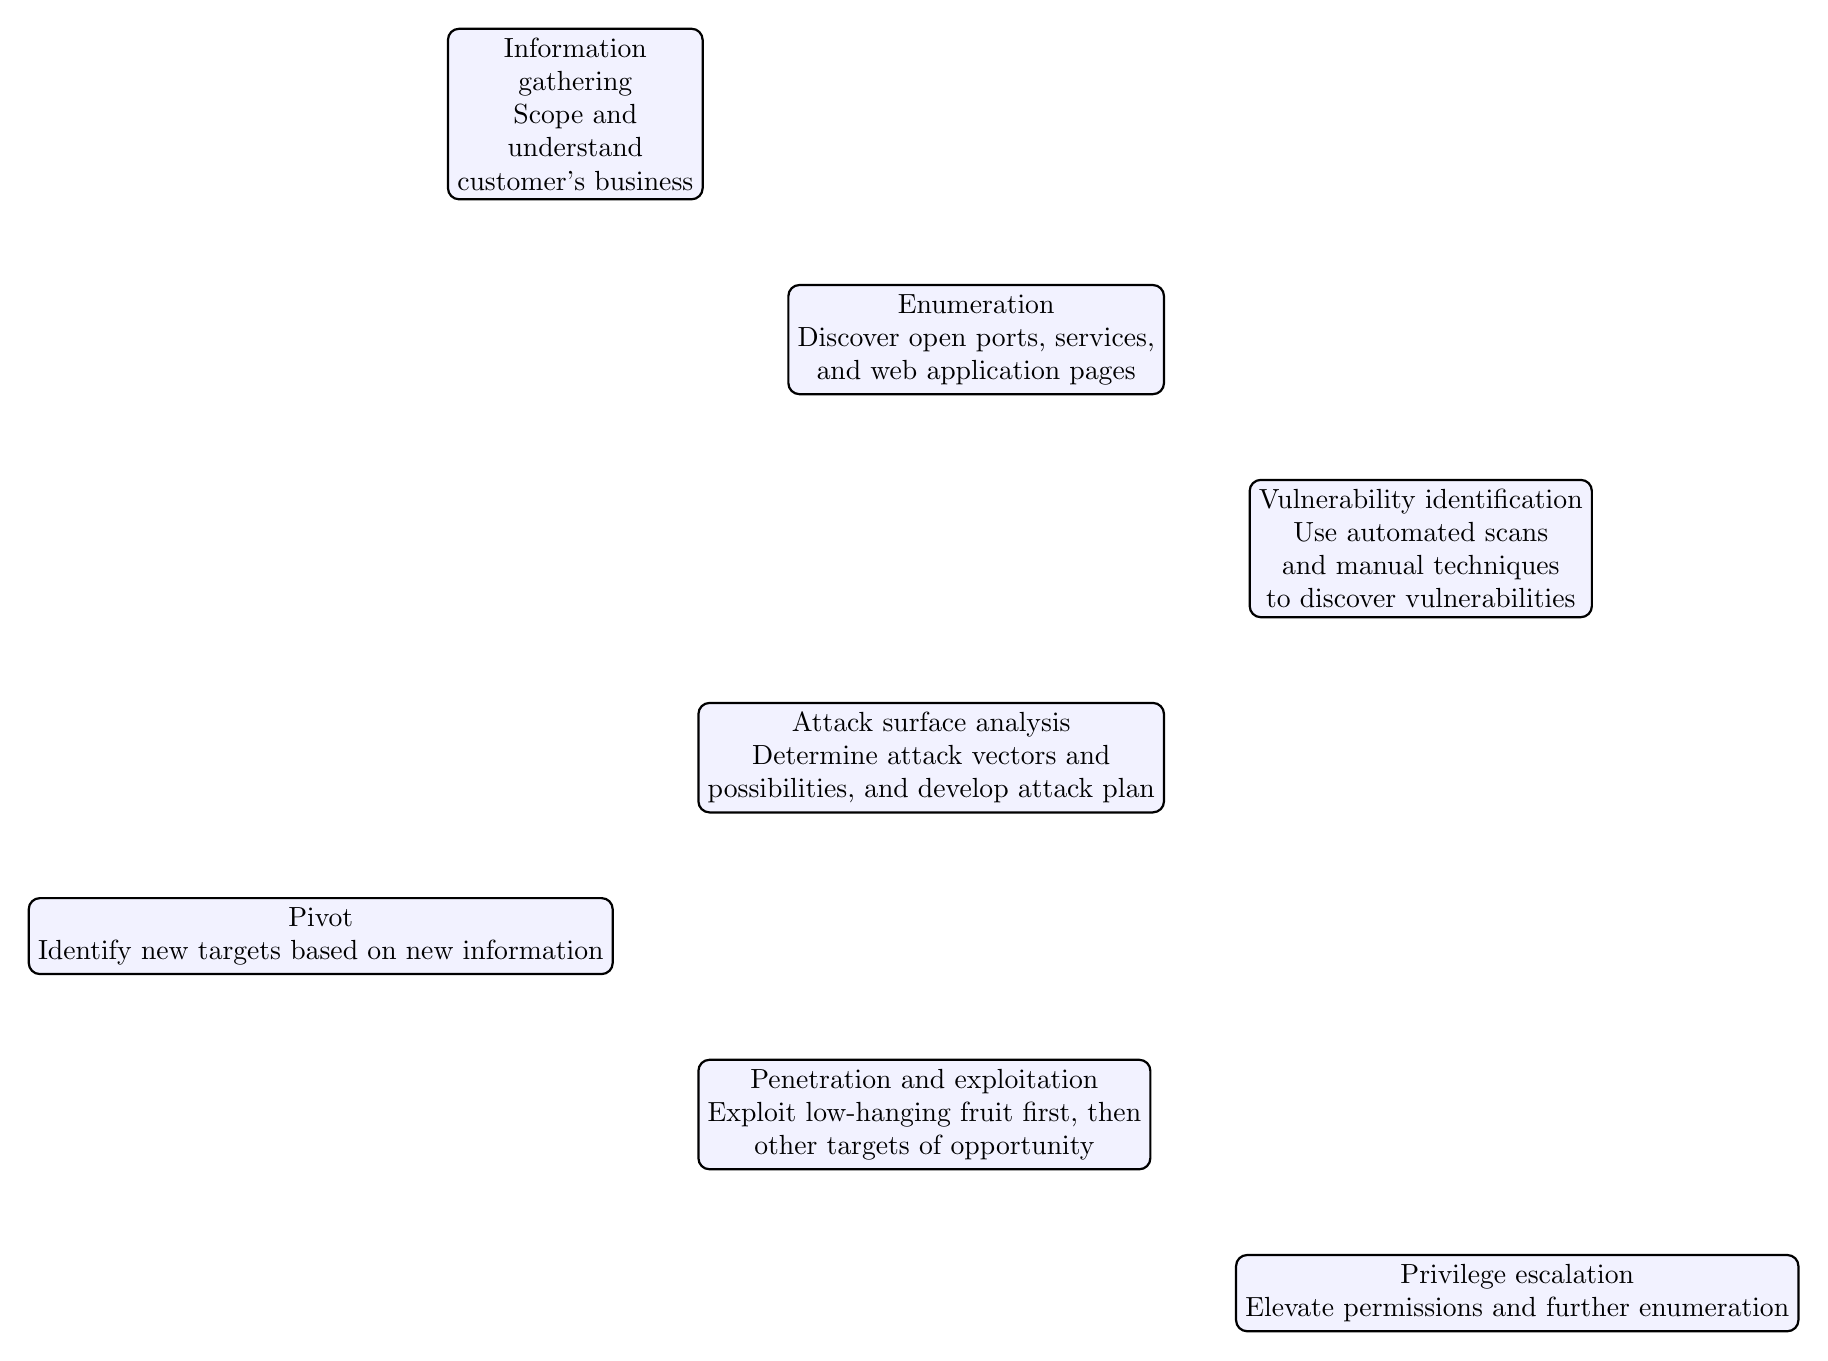
\begin{tikzpicture}[node distance=1.5cm, auto]
            \node[block, align=center, text width=3cm] (info) {Information gathering\\Scope and understand\\customer's business};
            \node[block, align=center, below right=of info] (enum) {Enumeration\\Discover open ports, services,\\and web application pages};
            \node[block, align=center, below right=of enum] (vuln) {Vulnerability identification\\Use automated scans\\and manual techniques\\to discover vulnerabilities};
            \node[block, align=center, below left=of vuln] (attack) {Attack surface analysis\\Determine attack vectors and\\possibilities, and develop attack plan};
            \node[block, align=center, below left=of attack] (pivot) {Pivot\\Identify new targets based on new information};
            \node[block, align=center, below right=of pivot] (pen) {Penetration and exploitation\\Exploit low-hanging fruit first, then\\other targets of opportunity};
            \node[block, align=center, below right=of pen] (priv) {Privilege escalation\\Elevate permissions and further enumeration};

            \path[arrow] (info) -- (enum);
            \path[arrow] (enum) -- (vuln);
            \path[arrow] (vuln) -- (attack);
            \path[arrow] (attack) -- (pivot);
            \path[arrow] (pivot) -- (pen);
            \path[arrow] (pen) -- (priv);
            \path[arrow] (priv) -- (info);
        \end{tikzpicture}
    \end{adjustbox}
    \caption{Penetration Testing Stages - Detailed}
\end{figure}

\subsection{OWASP and the Top Ten}

The **Open Web Application Security Project (OWASP)** is a non-profit foundation dedicated to improving the security of software.  OWASP provides a wealth of resources, including tools, community forums, and educational materials.  One of OWASP's most valuable contributions is the **OWASP Top Ten**, a regularly updated list of the ten most common web application security flaws.  The Top Ten is released every 3-4 years and serves as a critical resource for developers and security professionals.  The current Top Ten (as of 2021) is categorized based on **exploitability**, **prevalence**, **detectability**, and **technical** impact.  Understanding these vulnerabilities is essential for building secure web applications.

\subsection{OWASP Top Ten (2021)}

The 2021 OWASP Top Ten represents a significant shift in focus compared to previous iterations.  Several new vulnerabilities have been added, and the ranking of existing vulnerabilities has changed.  Key changes include the addition of **Insecure Design** (A04:2021) and **Software and Data Integrity Failures** (A08:2021).  **Broken Access Control** (A01:2021) remains the most critical risk, followed by **Cryptographic Failures** (A02:2021) and **Injection** (A03:2021).  Other vulnerabilities on the list include **Security Misconfiguration** (A05:2021), **Vulnerable and Outdated Components** (A06:2021), **Identification and Authentication Failures** (A07:2021), **Security Logging and Monitoring Failures** (A09:2021), and **Server-Side Request Forgery (SSRF)** (A10:2021).

\begin{figure}[H]
    \centering
    \begin{adjustbox}{max width=\textwidth}
        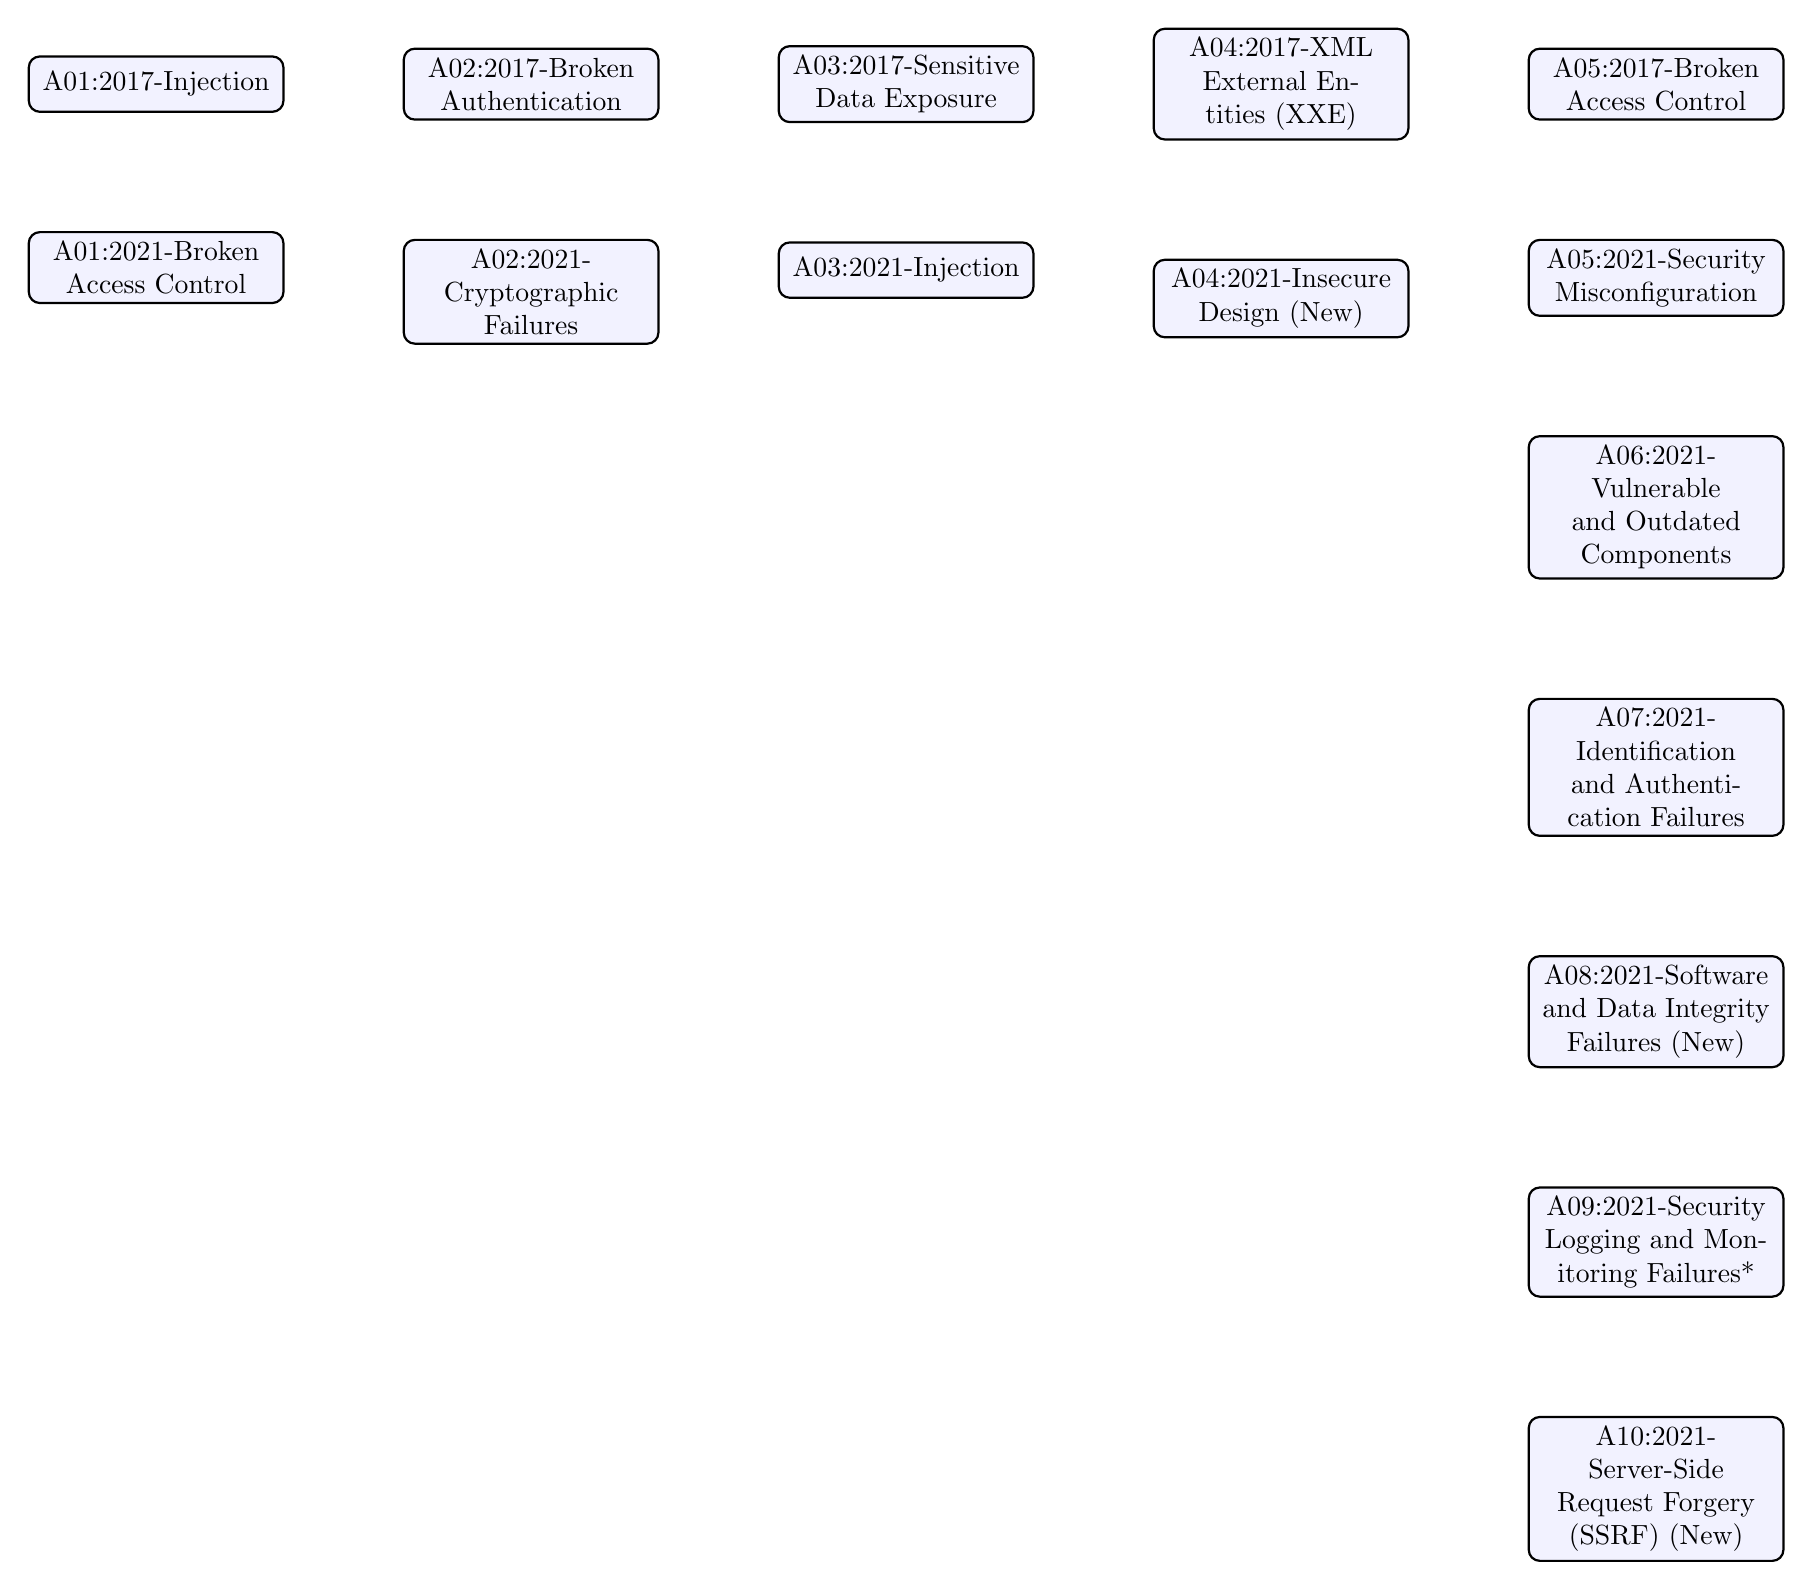
\begin{tikzpicture}[node distance=1.5cm, auto]
            \node[block, text width=3cm, align=center] (a01_17) {A01:2017-Injection};
            \node[block, text width=3cm, align=center, right=of a01_17] (a02_17) {A02:2017-Broken Authentication};
            \node[block, text width=3cm, align=center, right=of a02_17] (a03_17) {A03:2017-Sensitive Data Exposure};
            \node[block, text width=3cm, align=center, right=of a03_17] (a04_17) {A04:2017-XML External Entities (XXE)};
            \node[block, text width=3cm, align=center, right=of a04_17] (a05_17) {A05:2017-Broken Access Control};
            \node[block, text width=3cm, align=center, below=of a01_17] (a01_21) {A01:2021-Broken Access Control};
            \node[block, text width=3cm, align=center, below=of a02_17] (a02_21) {A02:2021-Cryptographic Failures};
            \node[block, text width=3cm, align=center, below=of a03_17] (a03_21) {A03:2021-Injection};
            \node[block, text width=3cm, align=center, below=of a04_17] (a04_21) {A04:2021-Insecure Design (New)};
            \node[block, text width=3cm, align=center, below=of a05_17] (a05_21) {A05:2021-Security Misconfiguration};
            \node[block, text width=3cm, align=center, below=of a05_21] (a06_21) {A06:2021-Vulnerable and Outdated Components};
            \node[block, text width=3cm, align=center, below=of a06_21] (a07_21) {A07:2021-Identification and Authentication Failures};
            \node[block, text width=3cm, align=center, below=of a07_21] (a08_21) {A08:2021-Software and Data Integrity Failures (New)};
            \node[block, text width=3cm, align=center, below=of a08_21] (a09_21) {A09:2021-Security Logging and Monitoring Failures*};
            \node[block, text width=3cm, align=center, below=of a09_21] (a10_21) {A10:2021-Server-Side Request Forgery (SSRF) (New)};

            \path[arrow] (a01_17) -- (a01_21);
            \path[arrow] (a02_17) -- (a02_21);
            \path[arrow] (a03_17) -- (a03_21);
            \path[arrow] (a04_17) -- (a04_21);
            \path[arrow] (a05_17) -- (a05_21);
        \end{tikzpicture}
    \end{adjustbox}
    \caption{OWASP Top Ten - 2017 vs. 2021}
\end{figure}

\subsection{A1: Broken Access Control}

**Broken Access Control** refers to flaws in a system that allow users to access resources or perform actions that they are not authorized to.  Access control mechanisms are designed to enforce policies that restrict users to their intended permissions.  When these mechanisms fail, it can lead to unauthorized information disclosure, modification, or destruction of data, or the ability to perform business functions outside the user's limits.  This is a critical vulnerability because it can have a significant impact on the confidentiality, integrity, and availability of a system.


% --- START OF CHUNK 2 ---

\section{Vulnerabilities}

A robust security posture requires a thorough understanding of potential vulnerabilities. Several common weaknesses can compromise the integrity and confidentiality of a system. A fundamental principle is that of **least privilege**, meaning users should only have access to the resources they absolutely need to perform their duties.  Denying access by default, and then explicitly granting permissions, is a core tenet of secure system design.  Violations of this principle significantly expand the attack surface.

Another common vulnerability arises from improper access control checks. Attackers may attempt to **bypass** these controls by directly manipulating the URL, a technique known as **parameter tampering**. This often involves modifying parameters passed in the URL to gain unauthorized access to resources or functionality.

Permitting unauthorized viewing or editing of another user's account is a severe security flaw. This can lead to data breaches, identity theft, and other malicious activities. Similarly, APIs lacking proper access controls for operations like `POST`, `PUT`, and `DELETE` are vulnerable to abuse.  An attacker could potentially create, modify, or delete data without authorization.

**Elevation of privilege** is a critical vulnerability where a user gains access to functionalities or data they are not authorized to access. This can occur even without being logged in, indicating a flaw in the authentication or authorization mechanisms.

Modern web applications often rely on **JSON Web Tokens (JWTs)** for authentication and authorization.  However, these tokens are susceptible to **metadata manipulation**, such as replay attacks (where a valid token is reused) or tampering (where the token's contents are altered).  Proper validation and secure storage of JWTs are essential.

Finally, vulnerabilities can exist that allow attackers to force browsing to authenticated pages as an unauthenticated user, or to privileged pages as a standard user. This often exploits weaknesses in session management or access control logic.

\section{Web HTTP Methods}

The foundation of communication on the web relies on **HTTP Methods**, which define the type of operation being performed. These methods dictate how data is sent back and forth between the client (e.g., a web browser) and the server. Understanding these methods is crucial for both web development and security analysis.

\textbf{GET} requests are used to **retrieve** data from the server. They are typically used for read-only operations and should not be used to modify data.

\textbf{PUT} requests are used to **send updated** data to the server, effectively replacing an existing resource.

\textbf{POST} requests are used to **send new** or **created** data to the server, often resulting in the creation of a new resource.

\textbf{DELETE} requests are used to **remove** data from the server.

\section{HTTP Status Codes}

When a client sends a request to a server, the server responds with an **HTTP Status Code** indicating the outcome of the request. These codes provide valuable information about the success or failure of the operation.

Codes beginning with **20X** indicate success. For example, **200 OK** signifies a successful request, **201 Created** indicates that a new resource was successfully created, and **204 No Content** indicates that the request was successful, but there is no content to return.

Codes beginning with **30X** indicate redirection. **301 Moved Permanently** indicates that the requested resource has been permanently moved to a new location, and **304 Not Modified** indicates that the client's cached version of the resource is still valid.

Codes beginning with **40X** indicate client errors. **400 Bad Request** signifies that the server could not understand the request, **401 Unauthorized** indicates that authentication is required, **403 Forbidden** indicates that the client does not have permission to access the resource, and **404 Not Found** indicates that the requested resource could not be found.

Codes beginning with **50X** indicate server errors. **500 Internal Server Error** signifies a generic server error, and **503 Service Unavailable** indicates that the server is temporarily unavailable.

\section{How to Prevent Vulnerabilities}

Proactive security measures are essential to mitigate the risks associated with the vulnerabilities discussed earlier. A key principle is to **deny by default**, granting access only when explicitly required.

Implementing **Cross-Origin Resource Sharing (CORS)** is crucial for controlling which domains are allowed to access resources from your web application. This helps prevent cross-site scripting (XSS) attacks.

Disabling **web server directory listing** prevents attackers from discovering sensitive files and directories by simply browsing the server.

**Logging access control failures** and regularly reviewing these logs can help identify and address potential security breaches.

It is vital to ensure that the **correct user** is making any changes to the system. Utilizing **tokens for authentication**, such as JWTs, provides a secure and standardized way to verify user identity.  A resource like \href{https://jwt.io}{https://jwt.io} provides information and tools for working with JWTs.

Finally, making **IDs harder to guess** (e.g., using non-numeric values) can prevent attackers from predicting and exploiting valid IDs. Tools like \href{https://guidgenerator.com/}{https://guidgenerator.com/} can generate universally unique identifiers (GUIDs).

\section{Cryptographic Failures}

**Cryptographic Failures**, previously known as **Sensitive Data Exposure**, represent a significant security risk. This category encompasses vulnerabilities related to the protection of data both **in transit** (while being transmitted over a network) and **at rest** (while being stored).

Protecting sensitive data such as **passwords**, **credit card numbers**, **health records**, and **personally identifiable information (PII)** is paramount.  Failure to do so can result in severe consequences, including financial loss, reputational damage, and legal penalties.

More information on this topic can be found at \href{https://owasp.org/www-project-top-ten/OWASP_Top_Ten_2017/Top_10-2017_A3-Sensitive_Data_Exposure}{https://owasp.org/www-project-top-ten/OWASP_Top_Ten_2017/Top_10-2017_A3-Sensitive_Data_Exposure}.

\section{Identifying Cryptographic Vulnerabilities}

Determining whether an application is vulnerable to cryptographic failures requires careful assessment. Several key questions should be addressed:

Is any data being transmitted in **clear text**? This is a major security risk, as the data can be intercepted and read by anyone with access to the network.

What **version of cryptography** is being used? Older algorithms like SHA1 and MD5 are known to be vulnerable to attacks and should be replaced with more secure alternatives.

Are the **default crypto keys** in use? Default keys are often weak and easily compromised. It is essential to generate strong, unique keys.

Is the **certificate chain** from the Certificate Authority (CA) validated? An invalid or expired certificate can indicate a man-in-the-middle attack.

Are the **same keys** being used on multiple servers? This can increase the risk of compromise, as a single key breach can affect multiple systems.

\section{Classifying Data}

Before implementing security measures, it is crucial to **classify data** based on its sensitivity. This involves determining the potential impact of a data breach and the legal or regulatory requirements that apply.

Consider these questions:

Is it a **company secret**?
Are there **legal requirements** for protecting the data?
Is it someone's **Personally Identifiable Information (PII)**?
Is it someone's **Health Data (HIPAA)**?
Is it a **Password, PIN code, or Security Question Answer**?

\subsection{Data Storage and Transmission}

Once data has been classified, the appropriate storage and transmission methods can be determined.

\textbf{Passwords and PIN codes} should always be **hashed** using a strong hashing algorithm.

\textbf{User personal information} and \textbf{user health information} should be **encrypted** both in transit and at rest.

\textbf{Company private information} should also be **encrypted**.

\textbf{Company public information} and \textbf{user public information} can be stored in **plain text**, as they are not considered sensitive.

\section{Secure Data Transmission}

Secure data transmission is essential to protect data in transit.

\textbf{HTTP (Web)} is inherently insecure and should always be replaced with **HTTPS (Secure Web)**, which uses encryption to protect data.

\textbf{FTP (File Transfer)} is also insecure and should be replaced with **FTPS (Secure File Transfer)**.

\textbf{SMTP (Mail)} is not secure by default. While there is no universally secure mail protocol, many mail programs and online solutions (e.g., Gmail) offer encryption and decryption capabilities.

\section{Secure Email}

While SMTP lacks inherent security, secure email communication is possible through the use of **add-ons** for email clients. These add-ons typically implement **public key encryption**, where both the sender and receiver have a public key to encrypt messages and a private key to decrypt them.

However, public key encryption requires **coordination between both parties** to exchange public keys and ensure secure communication.


% --- START OF CHUNK 3 ---

\section{Credit Cards and Data Security}

\subsection{PCI Standards}
The **Payment Card Industry (PCI)** has established a comprehensive set of standards that organizations must adhere to when storing, processing, or transmitting **cardholder data**. These standards are designed to protect sensitive information and prevent fraud. A key principle within these standards is a discouragement of storing credit card data whenever possible. This is due to the inherent risks associated with maintaining such sensitive information, including the potential for data breaches and the significant compliance burden. 

For businesses that require recurring payments, the recommended approach is to utilize a **token** provided by a credit card clearing company, such as First Data. A token is an encrypted representation of the cardholder data, replacing the actual sensitive information with a non-sensitive equivalent. This significantly reduces the risk of a data breach, as the actual credit card details are never stored on the merchant's systems.

\subsection{Data Storage Best Practices}
Minimizing the storage of sensitive data is paramount in maintaining a strong security posture.  The principle of **least privilege** applies here – only store data that is absolutely necessary. When sensitive data *must* be stored, several techniques can be employed to mitigate risk. **Data truncation** involves shortening the data, such as displaying only the last four digits of a **Social Security Number (SSN)**. This limits the exposure of the full sensitive value while still allowing for identification purposes. 

**Encryption** is a critical security measure. At a minimum, any sensitive data that must be stored should be encrypted both in transit and at rest.  Furthermore, consider moving sensitive data to a separate, internal system that is specifically designed for secure data storage, if your primary web application does not require direct access to it.  For data that needs to be compared or matched but does not need to be displayed in its original form, **hashing** is an excellent option. Hashing transforms the data into a one-way, irreversible string of characters, protecting the original value.

\subsection{Preventative Measures}
Proactive security measures are essential for protecting sensitive data.  A fundamental step is to **classify data** based on its sensitivity level. This classification should inform the security controls applied to the data.  It's crucial to remember that data classification must also take into account relevant **laws and regulations**, such as GDPR, CCPA, or HIPAA, which may impose specific requirements for handling certain types of data. 

Beyond classification, consistently apply the principle of not storing sensitive data unless absolutely necessary.  All sensitive data at rest should be encrypted using strong, up-to-date **cryptography**.  Ensure that your systems are configured to use **TLS 1.2 or above** for secure communication. Finally, **disable caching** of sensitive data to prevent accidental exposure.

\section{Injection Attacks}

\subsection{Understanding Injection Attacks}
**Injection attacks** are a common web security vulnerability that occurs when untrusted data is sent to an interpreter as part of a command or query. The most prevalent type of injection attack is **SQL injection**, but other forms include **NoSQL injection**, **command injection**, **OS command injection**, and **LDAP injection**.  These attacks exploit vulnerabilities in how applications handle user input, allowing attackers to manipulate the application's logic and potentially gain unauthorized access to data or systems.

Injection attacks are successful when an application fails to properly **validate** or **sanitize** user-supplied data before using it in a query or command. This allows attackers to inject malicious code that is then executed by the application.

\subsection{Identifying Vulnerable Applications}
Several indicators suggest that an application may be vulnerable to injection attacks. These include:

\begin{itemize}
    \item **Unvalidated User Input:** The application directly uses user-supplied data without proper validation or sanitization.
    \item **Dynamic Queries:** The application constructs queries dynamically by concatenating user input with SQL code.
    \item **Direct Data Usage:** Hostile data is directly used or concatenated into the input without any filtering or escaping.
\end{itemize}

\subsection{Relational Databases}
**Relational databases** are a highly efficient method for storing and managing data. They organize data into **tables**, which consist of **columns** and **rows**, similar to a spreadsheet. This structured approach allows for efficient querying and manipulation of data.  Data within these tables is accessed and managed using **Structured Query Language (SQL)**.

\subsection{Relational Database Options}
There are numerous relational database options available, both free and commercial. Some popular choices include:

\begin{itemize}
    \item \textbf{Free:} **MySQL** and **PostgreSQL** are open-source relational databases that offer robust features and performance.
    \item \textbf{Enterprise:} **Microsoft SQL Server**, **Oracle Database**, and **IBM DB2** are commercial databases that provide advanced features, scalability, and support.
\end{itemize}

\begin{figure}[H]
    \centering
    \begin{adjustbox}{max width=\textwidth}
        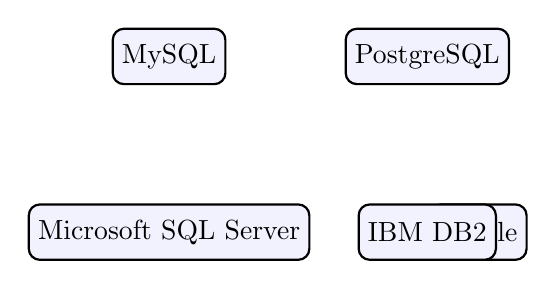
\begin{tikzpicture}[node distance=1.5cm, auto]
            \node[block] (mysql) {MySQL};
            \node[block, right=of mysql] (postgres) {PostgreSQL};
            \node[block, below=of mysql] (mssql) {Microsoft SQL Server};
            \node[block, right=of mssql] (oracle) {Oracle};
            \node[block, below=of postgres] (ibm) {IBM DB2};
        \end{tikzpicture}
    \end{adjustbox}
    \caption{Popular Relational Database Options}
\end{figure}

\subsection{MySQL: A Closer Look}
**MySQL** is one of the most widely used **free** and open-source relational databases. It is owned by Oracle and provides server and management consoles for multiple operating systems, including Windows, macOS, and Unix.  MySQL is known for its ease of use, performance, and scalability, making it a popular choice for a wide range of applications. You can find more information at \href{https://www.mysql.com/}{https://www.mysql.com/}.

\subsection{Tables, Rows, and Columns}
In a relational database, every table is assigned a unique name, such as "Users" or "Products." Each table is composed of **columns**, which define the attributes of the data, and **rows**, which represent individual records. For example, a "Users" table might have columns for "Name," "Username," and "Email," with each row representing a different user.

\begin{figure}[H]
    \centering
    \begin{adjustbox}{max width=\textwidth}
        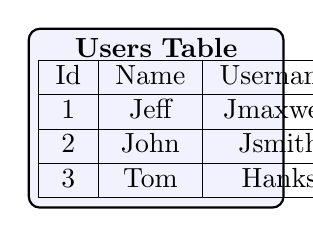
\begin{tikzpicture}[node distance=1.5cm, auto]
            \node[block, text width=3cm, align=center] (table) {
                \textbf{Users Table} \\
                \begin{tabular}{|c|c|c|c|c|}
                    \hline
                    Id & Name & Username & Email & Password \\ \hline
                    1 & Jeff & Jmaxwell & jmaxwell@okcu.edu & Password\#123 \\ \hline
                    2 & John & Jsmith & jsmith@okcu.edu & Password\#123 \\ \hline
                    3 & Tom & Hanks & thanks@okcu.edu & Password\#123 \\ \hline
                \end{tabular}
            };
        \end{tikzpicture}
    \end{adjustbox}
    \caption{Example of a Relational Database Table}
\end{figure}

\subsection{CRUD Operations}
Relational databases support the fundamental **CRUD** operations: **Create**, **Read**, **Update**, and **Delete**. These operations allow you to manage data within the database. In **SQL**, these operations are represented by the following keywords:

\begin{itemize}
    \item \textbf{Create} = \texttt{INSERT INTO}
    \item \textbf{Read} = \texttt{SELECT}
    \item \textbf{Update} = \texttt{UPDATE}
    \item \textbf{Delete} = \texttt{DELETE}
\end{itemize}


% --- START OF CHUNK 4 ---

\section{SQL: Read, Create, Update, and Delete Operations}

\subsection{Reading Data with SELECT}

The foundation of interacting with a database is the ability to **read** data. In SQL, this is accomplished using the \textbf{SELECT} statement. The basic syntax is straightforward: \texttt{SELECT [columns] FROM [table]}.  The \texttt{[columns]} portion specifies which data fields you want to retrieve. You can request specific columns, a comma-delimited list of columns, or use the wildcard character \texttt{*}, which instructs the database to return all columns in the specified \texttt{[table]}.  

For example, \texttt{SELECT * FROM Users} will return every column and every row from the \texttt{Users} table.  Conversely, \texttt{SELECT Name, Email FROM Users} will only return the \texttt{Name} and \texttt{Email} columns for all rows in the \texttt{Users} table.  This selective retrieval is crucial for efficiency, as it minimizes the amount of data transferred and processed.

\subsection{Filtering Data with the WHERE Clause}

Often, you don't need *all* the data in a table; you only need rows that meet specific criteria. This is where the \textbf{WHERE} clause comes into play. It allows you to filter rows based on conditions applied to specific columns. The general syntax is: \texttt{SELECT [columns] FROM [table] WHERE [column] = [value]}.  

The \texttt{[column]} represents the field you want to filter on, and the \texttt{[value]} is the condition that must be met.  For instance, \texttt{SELECT * FROM Users WHERE Name='Jeff'} will return only the rows from the \texttt{Users} table where the \texttt{Name} column is exactly equal to 'Jeff'.  The equality operator (=) is just one of many comparison operators available in SQL; others include >, <, >=, <=, and != (not equal to).

\subsection{Advanced WHERE Clause Examples}

The \textbf{WHERE} clause can be extended to handle more complex filtering scenarios.  One common technique is using the \textbf{LIKE} operator for pattern matching.  \texttt{SELECT * FROM Users WHERE Name LIKE 'J\%'} will return all users whose names begin with the letter 'J'. The \texttt{\%} symbol is a wildcard character representing zero or more characters.  

Another example is filtering by a specific ID: \texttt{SELECT * FROM Users WHERE Id=2}. This will retrieve the row where the \texttt{Id} column has a value of 2.  These examples demonstrate the power and flexibility of the \textbf{WHERE} clause in refining your data queries.

\subsection{Creating Data with INSERT INTO}

While \textbf{SELECT} retrieves data, \textbf{INSERT INTO} allows you to add new data to a table. The syntax is: \texttt{INSERT INTO [table] ([columns]) VALUES ([values])}.  You specify the \texttt{[table]} you want to insert into, the \texttt{[columns]} you're providing values for, and the corresponding \texttt{[values]} themselves.  

It's important to maintain the correct order and data types when specifying values.  For example, \texttt{INSERT INTO Users (Id, Name, Email,....) VALUES (4, ‘Hank', 'hank@okcu.edu',....)} inserts a new user with an ID of 4, the name 'Hank', and the email address 'hank@okcu.edu', along with any other specified column values.

\subsection{Updating Data with UPDATE}

Sometimes, you need to modify existing data. The \textbf{UPDATE} statement allows you to do this. The syntax is: \texttt{UPDATE [table] SET [column]=[value] WHERE [column]=[value]}.  You specify the \texttt{[table]} to update, the \texttt{[column]} you want to change, the new \texttt{[value]} for that column, and crucially, a \textbf{WHERE} clause to identify which rows to update.

**Caution:**  If you omit the \textbf{WHERE} clause, *all* rows in the table will be updated with the new value, which is rarely the desired outcome.  For example, \texttt{UPDATE Users SET Name='Jeff Maxwell' WHERE Id=1} will change the name of the user with an ID of 1 to 'Jeff Maxwell'.

\subsection{Deleting Data with DELETE}

The \textbf{DELETE} statement removes rows from a table. The syntax is: \texttt{DELETE FROM [table] WHERE [column]=[value]}.  Similar to \textbf{UPDATE}, the \textbf{WHERE} clause is essential to specify which rows to delete.

**Extreme Caution:**  Deleting data is a permanent operation.  If you omit the \textbf{WHERE} clause, *all* rows in the table will be deleted, and this action is generally irreversible.  Therefore, always double-check your \textbf{WHERE} clause before executing a \textbf{DELETE} statement.  For example, \texttt{DELETE FROM Users WHERE Id=1} will remove the user with an ID of 1 from the \texttt{Users} table.

\subsection{Example SQL Query and Data}

Let's consider a simple \texttt{Users} table with the following data:

\begin{figure}[H]
    \centering
    \begin{adjustbox}{max width=\textwidth}
        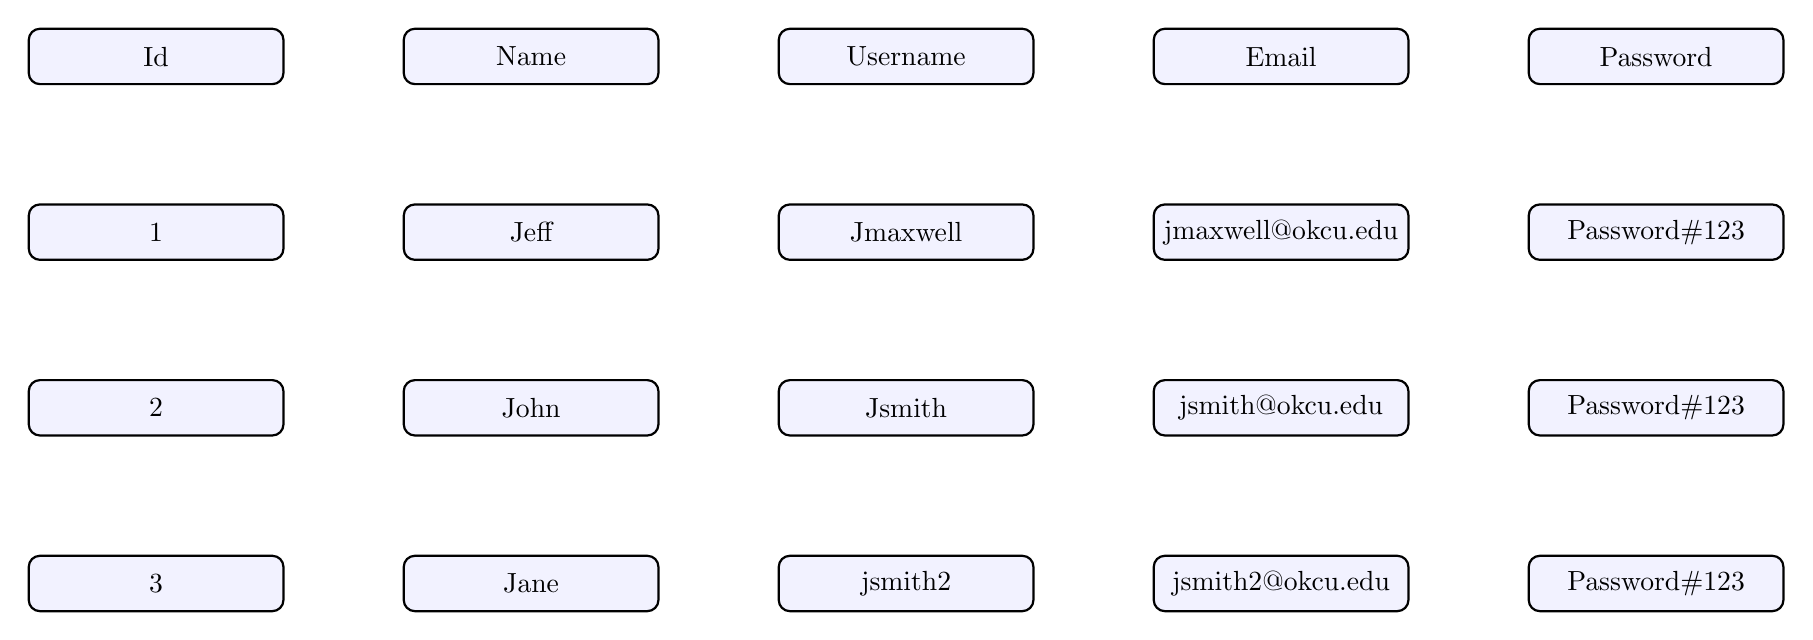
\begin{tikzpicture}[node distance=1.5cm, auto]
            \node[block, text width=3cm, align=center] (id) {Id};
            \node[block, text width=3cm, align=center] (name) [right=of id] {Name};
            \node[block, text width=3cm, align=center] (username) [right=of name] {Username};
            \node[block, text width=3cm, align=center] (email) [right=of username] {Email};
            \node[block, text width=3cm, align=center] (password) [right=of email] {Password};

            \node[block, text width=3cm, align=center] (id1) [below=of id] {1};
            \node[block, text width=3cm, align=center] (name1) [right=of id1] {Jeff};
            \node[block, text width=3cm, align=center] (username1) [right=of name1] {Jmaxwell};
            \node[block, text width=3cm, align=center] (email1) [right=of username1] {jmaxwell@okcu.edu};
            \node[block, text width=3cm, align=center] (password1) [right=of email1] {Password\#123};

            \node[block, text width=3cm, align=center] (id2) [below=of id1] {2};
            \node[block, text width=3cm, align=center] (name2) [right=of id2] {John};
            \node[block, text width=3cm, align=center] (username2) [right=of name2] {Jsmith};
            \node[block, text width=3cm, align=center] (email2) [right=of username2] {jsmith@okcu.edu};
            \node[block, text width=3cm, align=center] (password2) [right=of email2] {Password\#123};

            \node[block, text width=3cm, align=center] (id3) [below=of id2] {3};
            \node[block, text width=3cm, align=center] (name3) [right=of id3] {Jane};
            \node[block, text width=3cm, align=center] (username3) [right=of name3] {jsmith2};
            \node[block, text width=3cm, align=center] (email3) [right=of username3] {jsmith2@okcu.edu};
            \node[block, text width=3cm, align=center] (password3) [right=of email3] {Password\#123};
        \end{tikzpicture}
    \end{adjustbox}
    \caption{Example Users Table}
\end{figure}

Running the query \texttt{SELECT * FROM Users} would return all rows and columns from this table.

\section{SQL Injection: A Security Vulnerability}

\subsection{How SQL Injection Works}

\textbf{SQL injection} is a common web security vulnerability that allows attackers to interfere with the queries that an application makes to its database. It typically occurs when user input is improperly sanitized and is used directly in a SQL query.  A common scenario involves a login screen where a username and password are checked against a database.

An attacker can exploit this by adding malicious SQL code to the password field. For example, adding \texttt{OR X=X} to the end of the password. The result of \texttt{X=X} is always true, effectively bypassing the password check. If the code is not properly written to prevent this, the website may incorrectly believe the correct password has been entered.

\subsection{Example of SQL Injection}

Consider the following SQL query:

\texttt{SELECT * FROM Users WHERE username='jmaxwell' AND password='Password\#123';}

If the application directly concatenates user input into this query, an attacker could submit the following as the password: \texttt{‘Password\#123’ OR ‘1’='1’ --}.  This results in the following query:

\texttt{SELECT * FROM Users WHERE username='jmaxwell' AND password='Password\#123' OR ‘1’='1’ --';}

The \texttt{--} is a SQL comment, which effectively ignores the rest of the original query.  The \texttt{‘1’='1’} condition is always true, so the query will return all rows from the \texttt{Users} table, granting the attacker access.


% --- START OF CHUNK 5 ---

\section{Insecure Design}

\subsection{Introduction to Insecure Design (A04:2021)}

Insecure design represents a significant and broad category of vulnerabilities, newly highlighted in the OWASP Top Ten for 2021. It encompasses flaws stemming from fundamental weaknesses in the application's architecture and design choices.  This isn't about implementation errors (like coding mistakes); it's about problems inherent in *how* the system was conceived.  Common issues include **missing or ineffective control designs**, where security mechanisms are either absent or fail to adequately protect sensitive data and functionality.  Crucially, identifying insecure designs requires asking key questions: What are the potential **risks** associated with the current design? And, perhaps more importantly, how are those risks being **managed** – or, more accurately, *should* they be managed differently?  Addressing insecure design requires a proactive, holistic approach, shifting security considerations to the very beginning of the software development lifecycle (SDLC).

\subsection{What is Secure Design?}

Secure design is far more than simply creating a diagram that *includes* security elements. It represents a fundamental shift in **thinking, culture, and approach** to building both software and hardware systems. It's about embedding security as a core principle, not an afterthought.  This means moving beyond checklists and towards a mindset where security is considered at every stage, from initial concept to final deployment.  

Effective secure design necessitates the adoption of robust **methodologies** and a continuous, organization-wide commitment to improvement.  It requires a constant drive, originating from the highest levels of the corporation, to prioritize security and integrate it seamlessly into the design process.  This isn't a one-time fix; it's an ongoing evolution.

\subsection{Threat Modeling}

**Threat modeling** is a crucial practice in secure design. It involves systematically reviewing application diagrams and designs to proactively identify potential security issues.  Instead of waiting for vulnerabilities to be discovered during testing or, worse, in production, threat modeling allows developers to anticipate and mitigate risks *before* they become exploitable.  

The process involves asking critical questions about the system's architecture: How does **data flow** through the application? Is **encryption** being used to protect sensitive information, both in transit and at rest? And, fundamentally, who has **access to what** – and is that access appropriately controlled?  

\begin{figure}[H]
    \centering
    \begin{adjustbox}{max width=\textwidth}
        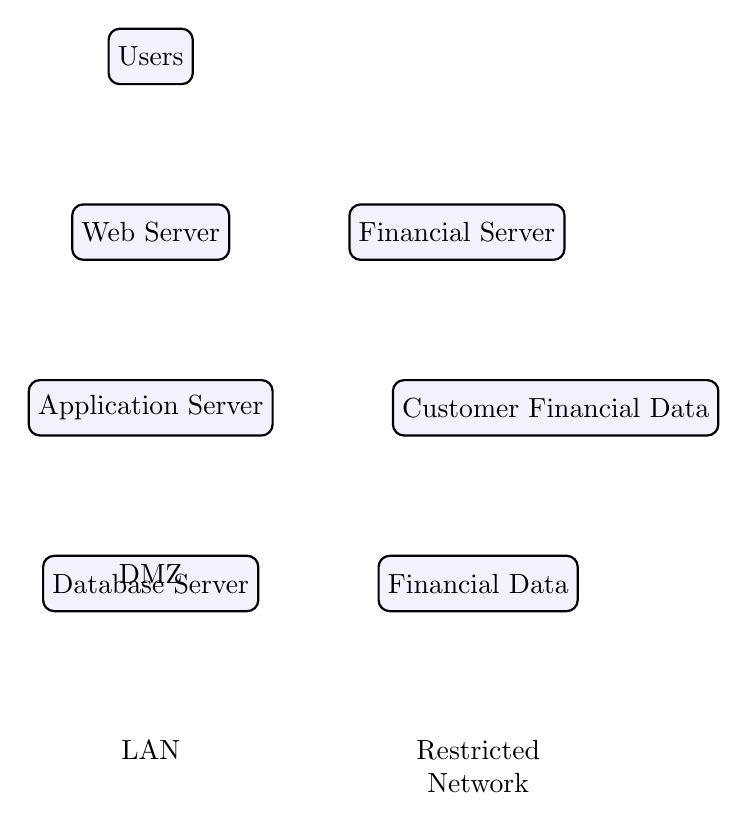
\begin{tikzpicture}[node distance=1.5cm, auto]
            \node[block] (users) {Users};
            \node[block, below=of users] (webserver) {Web Server};
            \node[block, right=of webserver] (financialserver) {Financial Server};
            \node[block, below=of webserver] (applicationserver) {Application Server};
            \node[block, below=of applicationserver] (databaseserver) {Database Server};

            \node[block, right=of applicationserver] (customerdata) {Customer Financial Data};
            \node[block, right=of databaseserver] (financialdata) {Financial Data};

            \path[arrow] (users) -- (webserver);
            \path[arrow] (webserver) -- (applicationserver);
            \path[arrow] (applicationserver) -- (databaseserver);
            \path[arrow] (databaseserver) -- (financialdata);
            \path[arrow] (webserver) -- (financialserver);
            \path[arrow] (applicationserver) -- (customerdata);

            \node[text width=2cm, align=center, below=of applicationserver] (dmz) {DMZ};
            \node[text width=2cm, align=center, below=of databaseserver] (lan) {LAN};
            \node[text width=2cm, align=center, below=of financialdata] (restrictednetwork) {Restricted Network};
        \end{tikzpicture}
    \end{adjustbox}
    \caption{Example Data Flow Diagram}
\end{figure}

\begin{figure}[H]
    \centering
    \begin{adjustbox}{max width=\textwidth}
        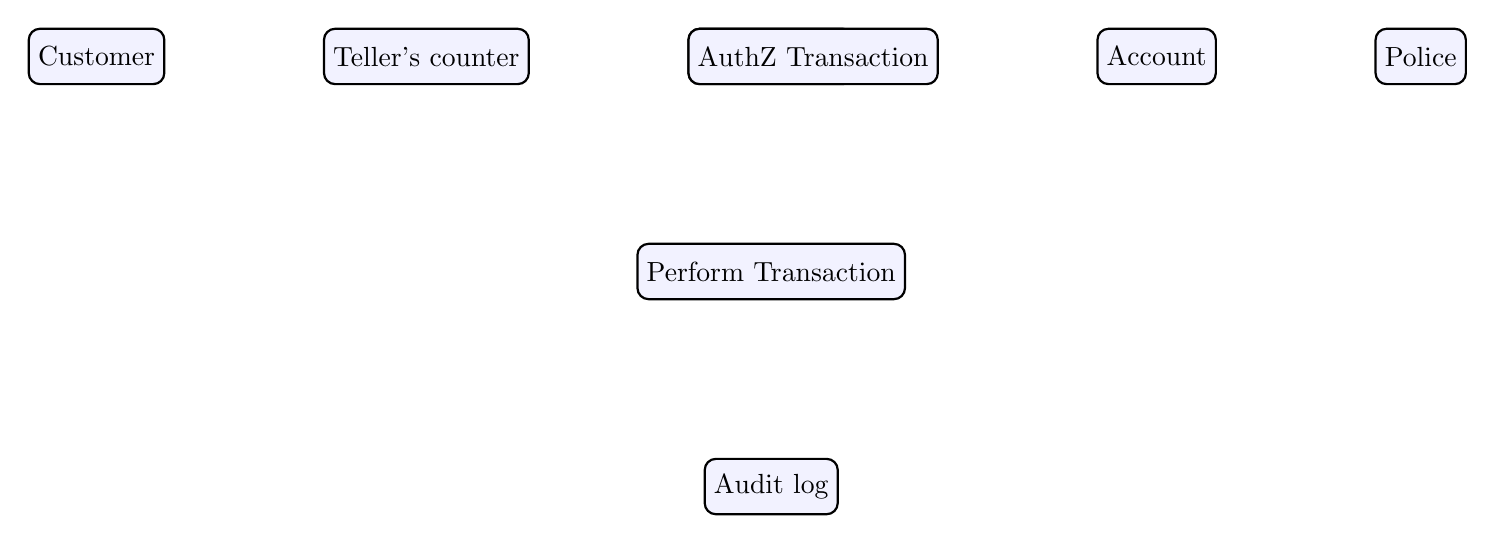
\begin{tikzpicture}[node distance=2cm, auto]
            \node[block] (customer) {Customer};
            \node[block, right=of customer] (teller) {Teller's counter};
            \node[block, right=of teller] (authnuser) {AuthN User};
            \node[block, below=of authnuser] (performtransaction) {Perform Transaction};
            \node[block, below=of performtransaction] (auditlog) {Audit log};
            \node[block, right=of teller] (authztransaction) {AuthZ Transaction};
            \node[block, right=of authztransaction] (account) {Account};
            \node[block, right=of account] (police) {Police};

            \path[arrow] (customer) -- (teller);
            \path[arrow] (teller) -- (authnuser);
            \path[arrow] (authnuser) -- (performtransaction);
            \path[arrow] (performtransaction) -- (auditlog);
            \path[arrow] (teller) -- (authztransaction);
            \path[arrow] (authztransaction) -- (account);
            \path[arrow] (account) -- (police);
        \end{tikzpicture}
    \end{adjustbox}
    \caption{Threat Modeling Example: Bank Withdrawal}
\end{figure}

\subsection{Data Considerations}

A thorough understanding of the data handled by the application is paramount to secure design.  Several key questions must be addressed: What specific **data** is being stored within the system? How is this data **classified** based on its sensitivity (e.g., public, confidential, restricted)? What data is being **hashed or encrypted**, and, crucially, *why* or *why not*?  The decision to encrypt should be based on a risk assessment, considering the potential impact of a data breach.  Who has **access to the data**, and are those access controls appropriately enforced?  Finally, what data is being **sent to other sources** (e.g., third-party vendors, cloud providers), and what security measures are in place to protect it during transmission and storage?

\subsection{Data Flow Analysis}

Analyzing **data flow** is a critical component of threat modeling and secure design.  This involves mapping how data moves between different systems and components within the application.  Key questions include: How does the data flow **between systems**? What are the specific **inputs and outputs** of each component? Is the data transferred in **plain text or cipher text**?  Using plain text is almost always unacceptable for sensitive data.  Finally, what **encryption methods** are being used for cipher text, and are those methods considered strong and up-to-date?  Outdated encryption algorithms can be easily broken, rendering the encryption ineffective.

\subsection{Security Assessment and Prevention}

Regular **security assessments** are essential for validating the effectiveness of secure design practices. Has a security assessment been performed on the application? When was the **last assessment** conducted? What were the **findings** of the assessment, and have those findings been addressed? How was the assessment **performed** – was it a manual penetration test, an automated vulnerability scan, or a combination of both?  

Organizations can also leverage frameworks like the **OWASP Software Assurance Maturity Model (SAMM)** (\url{https://owaspsamm.org}) to assess and improve their software security posture.

To **prevent** insecure designs, **AppSec (Application Security) professionals** must be actively involved in the design process from the outset, discussing security considerations early and often.  Building a **library of secure design patterns** and reference examples can provide developers with pre-approved, secure code snippets and architectural approaches.  Finally, consistently using **threat modeling** for critical systems and meticulously **diagramming/documenting data flows** are vital steps in creating more secure and resilient applications.


% --- START OF CHUNK 6 ---

\section{Preventing Common Attacks}

\subsection{Preventing SQL Injection, XSS, and CSRF}
To proactively defend against common web application vulnerabilities such as **SQL Injection**, **Cross-Site Scripting (XSS)**, and **Cross-Site Request Forgery (CSRF)**, a security-focused approach must be integrated throughout the software development lifecycle. This begins with the creation of detailed **User Stories** and **Requirements** that explicitly address these threats.  These stories should not simply state *what* the system should do, but also *how* it should do it securely.  For example, a user story might state, "As a user, I want to be able to search for products, ensuring that all user input is properly sanitized to prevent SQL injection attacks."  Following the creation of these stories, rigorous testing and validation of the system's design are crucial. This includes both static analysis (reviewing code for potential vulnerabilities) and dynamic analysis (testing the running application for vulnerabilities).  Finally, engaging a **Penetration Tester (PenTester)** – a security professional who attempts to exploit vulnerabilities in the system – provides a real-world assessment of the application's security posture.  A PenTester's report will highlight weaknesses that may have been missed during internal testing and provide valuable insights for remediation.

\section{Security Misconfiguration}

\subsection{Understanding Security Misconfiguration}
**Security Misconfiguration** is a pervasive vulnerability that arises from systems and software not being properly set up. This often stems from using default configurations, failing to patch known flaws, or leaving unnecessary services running. Attackers actively seek out these misconfigurations because they represent low-hanging fruit – easily exploitable weaknesses that can provide access to sensitive data or systems.  They frequently target **unpatched flaws** that have already been publicly disclosed, as many organizations are slow to apply security updates.  Furthermore, attackers will scan for **unprotected files and folders** containing sensitive information, such as configuration files or backups.

\subsection{Common Misconfiguration Issues}
Several specific misconfiguration issues are commonly observed:

\begin{itemize}
    \item \textbf{Lack of OS/System Hardening:}  Operating systems and applications often come with default settings that are not secure.  **Hardening** involves modifying these settings to reduce the attack surface and improve security.
    \item \textbf{Missing Latest Patches or Security Patches:} Regularly applying security patches is essential to address known vulnerabilities.  Failure to do so leaves systems exposed to exploitation.
    \item \textbf{Services Running That Shouldn't Be:}  Many systems run unnecessary services that provide potential attack vectors.  Disabling these services reduces the risk.
    \item \textbf{Features Installed That Need to Be Removed:}  Similar to unnecessary services, unused features can introduce vulnerabilities.  Removing them simplifies the system and reduces the attack surface.
    \item \textbf{Open Ports or Protocols:}  Unnecessary open ports and protocols provide potential entry points for attackers.  Closing these ports reduces the risk.
    \item \textbf{Error Handling That Shows Stack Trace with Security Information:}  Detailed error messages, especially those including **stack traces**, can reveal sensitive information about the system's internal workings, aiding attackers in identifying vulnerabilities.
    \item \textbf{Default Settings Sometimes Allow Too Much Access:} Default usernames, passwords, and permissions often provide attackers with an easy way to gain access to systems.
\end{itemize}

\subsection{Why Does Misconfiguration Happen?}
Security misconfiguration often occurs due to a combination of factors.  A significant contributor is that many **system administrators** set up systems without fully understanding the implications of the **default values** that are configured. They may not realize that default credentials need to be changed or that certain services should be disabled.  Another issue is the lack of **automated tools** for patching systems.  Without automation, it's easy for systems to be missed during patching cycles.  Finally, the convenience of **default configurations** often leads administrators to simply accept them without proper review and customization.

\subsection{Preventing Security Misconfiguration}
To mitigate the risk of security misconfiguration, a proactive and systematic approach is required.  This includes:

\begin{itemize}
    \item \textbf{Hardening Servers:} Collaborate with administrators and network engineers to “harden” servers by locking them down and reducing the attack surface.
    \item \textbf{Removing Default Accounts:} Eliminate any default accounts with known credentials.
    \item \textbf{Removing Unused Services:} Disable or uninstall any services that are not essential for the system's operation.
    \item \textbf{Turning Off Unused Ports:} Close any unused network ports to prevent unauthorized access.
    \item \textbf{Adding Default Error Handling:} Implement robust error handling that does not reveal sensitive information to users.
    \item \textbf{Least Privilege Approach:}  Adopt a **least privilege** approach, granting users and processes only the minimum necessary permissions to perform their tasks.
    \item \textbf{Secure OS Images:} Create secure, pre-configured versions of operating systems that can be used as a baseline for new systems.
    \item \textbf{Security Testing and Automation:} Utilize security testing tools and automated patching systems to identify and address vulnerabilities proactively.
    \item \textbf{Logging and Monitoring:} Implement comprehensive logging and monitoring to detect and respond to security incidents.  Critically, logs must be *reviewed* regularly.
\end{itemize}

\section{Vulnerable and Outdated Components}

\subsection{The Problem of Vulnerable Components}
In modern software development, it is common practice to leverage a combination of **third-party components** to accelerate development and provide specialized functionality. However, these components often contain **vulnerabilities** that can be exploited by attackers.  These vulnerabilities can range from minor bugs to critical security flaws that allow attackers to gain control of the system.  The risk is compounded by the fact that many components are **outdated**, meaning they no longer receive security updates.

\subsection{Is Your Application Vulnerable?}
The unfortunate reality is that most applications are likely vulnerable to some extent.  If you use any third-party components, and if you are not regularly scanning for vulnerabilities, and if you are several versions behind on the frameworks or tools you use, your application is at risk.

\subsection{Why Do Vulnerabilities Exist in Components?}
A significant portion of third-party software is **Open Source**, hosted on platforms like GitHub and GitLab.  While this fosters collaboration and innovation, it also means that the responsibility for updating the software, scanning for vulnerabilities, and releasing new versions falls to the **author(s)** of the project.  If the project is not actively maintained, or if the author lacks the resources or motivation to address security issues, vulnerabilities may remain unpatched for extended periods.  Furthermore, even **commercial (paid for)** software is not immune to vulnerabilities, and vendors may be slow to release patches.

\subsection{Tools for Identifying Vulnerable Components}
Fortunately, several tools can help identify vulnerable components in your applications:

\begin{itemize}
    \item \textbf{National Vulnerability Database (NVD):} \url{https://nvd.nist.gov} – A comprehensive database of known vulnerabilities.
    \item \textbf{GitHub/GitLab Scanners:} Both platforms offer built-in vulnerability scanners that can identify vulnerable dependencies in your projects.
    \item \textbf{OWASP Dependency-Check:} \url{https://owasp.org/www-project-dependency-check/} – A free and open-source tool for identifying known vulnerabilities in project dependencies.
    \item \textbf{Snyk.io:} \url{https://snyk.io} – A commercial platform that provides vulnerability scanning and remediation tools.
\end{itemize}


% --- START OF CHUNK 7 ---

\section{NPM and Dependency Management}

\textbf{Node Package Manager (NPM)} is an essential tool for any JavaScript developer working with Node.js. It serves as both a package manager and a registry for open-source libraries and tools.  NPM simplifies the process of incorporating external code into your projects, managing dependencies, and ensuring project reproducibility.  Dependencies are the external packages your project relies on to function correctly.  Without a package manager, tracking and updating these dependencies would be a manual and error-prone process.

Several key NPM commands are crucial for maintaining a secure and up-to-date project.  `npm ls [package name]` allows you to check if a specific package is installed and its version. This is useful for verifying dependencies and identifying potential conflicts.  `npm audit` scans your project's dependency tree for known security vulnerabilities.  Running `npm audit fix` attempts to automatically update vulnerable packages to patched versions.  However, it's important to review the changes made by `npm audit fix` before committing them, as automatic updates can sometimes introduce breaking changes. Finally, `npm update` updates all packages in your `package.json` file to their latest versions, respecting the version ranges specified in your project.

\section{Preventing Dependency Vulnerabilities}

Proactive measures are vital to prevent dependency vulnerabilities from impacting your applications. A core principle is to **patch, patch, patch** – regularly updating your dependencies as part of your development cycle. This ensures you benefit from security fixes and bug improvements released by package maintainers.

Removing **unused dependencies** is another critical step. Unused code represents a potential attack surface, as it may contain vulnerabilities that are never exploited in your application but still present a risk.  This can be challenging, as determining whether a dependency is truly unused can require careful analysis of your codebase.

Integrating a **vulnerability scanner** into your **Continuous Integration/Continuous Deployment (CI/CD)** pipelines is highly recommended. These scanners automatically identify vulnerabilities in your dependencies during the build and deployment process, preventing vulnerable code from reaching production.

Finally, always prioritize using components from **official sources**. Avoid relying on unofficial or untrusted repositories, as they may contain malicious code.

\subsection{Best Practices for Dependency Management}

Maintaining a local repository of your project's dependencies can provide greater control and reliability. This allows you to pull updates and update the repository regularly, ensuring consistency across your development team.

Establishing **scheduled release updates** – whether quarterly, monthly, or weekly – enforces a consistent cadence for dependency updates. This prevents dependencies from becoming excessively outdated and reduces the risk of accumulating vulnerabilities.

It's also crucial to avoid letting your application's **frameworks** fall too far behind. Staying within one or two versions of the latest stable release minimizes compatibility issues and ensures you have access to the latest security patches.

\section{OWASP A07: Identification and Authentication Failures}

The **Open Web Application Security Project (OWASP)** identifies the top ten most critical web application security risks.  **A07: Identification and Authentication Failures** currently ranks as the seventh most critical risk (previously #2 in 2017). This shift reflects improvements in secure authentication practices and better management of authenticated users, but it remains a significant concern.

\textbf{Authentication} relates to the process of verifying a user's identity, often through session management or login mechanisms. Incorrectly implemented authentication can lead to attackers gaining unauthorized access to user accounts and sensitive data.  Specifically, vulnerabilities in session management, weak password policies, and inadequate multi-factor authentication can be exploited.

Hackers can exploit these weaknesses to **log in as other users** or **gain access to pages and systems they should not have access to**. This can result in data breaches, financial loss, and reputational damage.

\section{Common Authentication Vulnerabilities}

Several common vulnerabilities can lead to identification and authentication failures.

Does your application **permit automated attacks such as credential stuffing**? Credential stuffing involves using stolen usernames and passwords obtained from other breaches to attempt to log in to your application.  The scale of this threat is significant, with billions of accounts compromised in previous data breaches (see \url{https://haveibeenpwned.com/}).

Does your application **permit brute force or other automated attacks**? Brute force attacks involve systematically trying different passwords until the correct one is found.

Does your application **permit default, weak, or well-known passwords** such as "Password1" or "admin/admin"?  These passwords are easily guessed and represent a significant security risk.

Does your application **use weak forgot-password processes** – such as knowledge-based answers (e.g., "What is your mother's maiden name?")? These questions are often easily obtainable through social engineering or public records.

\section{Secure Authentication Practices}

How is login validated and managed in your application?

Using **plain text, encrypted, or hashed passwords without salt** is a critical security flaw (classified as **A02: 2021 Cryptographic Failures** by OWASP).  Plain text passwords are easily compromised, while encrypted passwords can be decrypted.  Hashing passwords with a salt provides a more secure method of storage.

**Not using multi-factor authentication (MFA)** significantly increases the risk of account compromise. MFA requires users to provide multiple forms of identification, making it much more difficult for attackers to gain access even if they have stolen a password.

Finally, **pages that don't validate the user session or validate access to a page** can allow attackers to bypass authentication controls and access restricted resources.

\subsection{Credential Stuffing in Detail}

\textbf{Credential stuffing} is a particularly prevalent attack vector. Hackers leverage stolen account credentials from data breaches on other websites and attempt to use them on your application.  Websites like \textit{Have I Been Pwned?} (\url{https://haveibeenpwned.com/}) demonstrate the sheer scale of compromised accounts.  Major breaches affecting companies like Adobe, Equifax, LinkedIn, Yahoo!, eBay, Marriott, and Heartland Payment Systems have resulted in billions of exposed credentials.

\subsection{Brute Force Attacks and Weak Passwords}

\textbf{Brute force attacks} involve systematically trying different passwords until the correct one is found.  Attackers often use lists of **commonly used passwords** obtained from previous breaches.  A list of commonly used passwords can be found here: \url{https://github.com/danielmiessler/SecLists/blob/master/Passwords/darkweb2017-top10000.txt}.

Systems that allow simple passwords are easy to exploit. Tools like **HASHCAT** can be used to crack passwords efficiently.

\subsection{Weak Forgot-Password Processes}

A weak **forgot-password process** can also be exploited. If a system emails a user their password in plain text, it exposes the password to potential interception.  Furthermore, if the system reveals whether an email address or username exists during the password reset process, attackers can use this information to enumerate valid accounts.

\subsection{Password Storage Best Practices}

\textbf{Plain text passwords} are unequivocally bad and should never be stored.  \textbf{Encrypted passwords} are slightly better, but encryption can be reversed.  The gold standard is to **always hash passwords with a \textbf{RANDOM salt} value for each user**.  Salting adds a unique random value to each password before hashing, making it much more difficult for attackers to crack passwords using precomputed tables (rainbow tables).


% --- START OF CHUNK 8 ---

\section{Fixing Broken Authentication}

\subsection{Addressing Authentication Vulnerabilities}

Broken authentication is a critical security flaw that can lead to unauthorized access to sensitive data and systems. Several measures can be implemented to mitigate these risks. First, enforcing **complex password requirements** is essential. This includes mandating a minimum length, requiring a mix of uppercase and lowercase letters, numbers, and special characters.  However, complexity alone is not sufficient; passwords should also be stored securely.  This is achieved by **hashing passwords with a random salt**.  Hashing transforms the password into an irreversible string of characters, and the salt—a unique random value for each password—prevents attackers from using precomputed tables of common password hashes (rainbow tables).

Furthermore, implementing an **account lockout** mechanism after a specified number of failed login attempts can deter brute-force attacks.  This temporarily disables the account, preventing further attempts.  A crucial layer of security is **multi-factor authentication (MFA)**. MFA requires users to provide multiple verification factors—something they know (password), something they have (security token or smartphone), or something they are (biometric data)—significantly reducing the risk of unauthorized access even if a password is compromised.

\subsection{Credential Stuffing Attacks}

\textbf{Credential stuffing} is a particularly insidious attack where attackers use lists of usernames and passwords obtained from data breaches on other websites to attempt logins on your system. Because many users reuse passwords across multiple sites, a breach on one platform can compromise accounts on others. To defend against this, it's vital to **keep track of the number of failed login attempts** and alert both the user and administrators when a threshold is exceeded. This can indicate an ongoing credential stuffing attack.  

Implementing **multi-factor authentication** is a highly effective countermeasure against credential stuffing, as even with valid credentials, the attacker would still need to bypass the second factor. MFA can take various forms, including email or text message verification codes, QR code scans, or the use of a dedicated **RSA token** (see Figure \ref{fig:rsa_token}).  It's also beneficial to encourage users to check if their credentials have been compromised in known data breaches using services like \href{https://haveibeenpwned.com/}{haveibeenpwned.com}.

\begin{figure}[H]
    \centering
    \begin{adjustbox}{max width=\textwidth}
        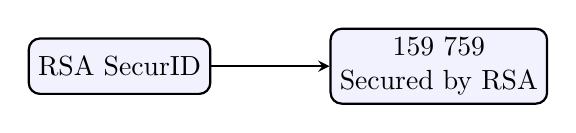
\begin{tikzpicture}[node distance=1.5cm, auto]
            \node[block] (rsa) {RSA SecurID};
            \node[block, right=of rsa] (display) {159 759 \\ Secured by RSA};
            \draw[arrow] (rsa) -- (display);
        \end{tikzpicture}
    \end{adjustbox}
    \caption{RSA SecurID Token}
    \label{fig:rsa_token}
\end{figure}

\subsection{Brute Force and Weak Password Attacks}

**Brute-force attacks** involve systematically trying every possible password combination until the correct one is found.  These attacks are often automated and can be successful against accounts with weak or easily guessable passwords. To mitigate this, maintain a **bad password list** and check new or changed passwords against it.  This list should include common passwords, dictionary words, and easily predictable patterns.

In addition to blocking known bad passwords, enforce **complex password rules**.  Specifically:
\begin{itemize}
    \item Passwords should be at least 8 characters long, with 15 or more being preferable.
    \item Passwords must contain both uppercase and lowercase letters.
    \item Passwords must include at least one special character (e.g., !@#$%^&*).
\end{itemize}

It's also important to consider password length.  A longer password, even if it doesn't meet strict complexity requirements, can be significantly harder to crack. For example, "Hello my name is Jeff Maxwell and I like to Teach #1 3 5" is more secure than "P@$$w0rd123", despite the latter containing special characters and numbers.

\begin{figure}[H]
    \centering
    \begin{adjustbox}{max width=\textwidth}
        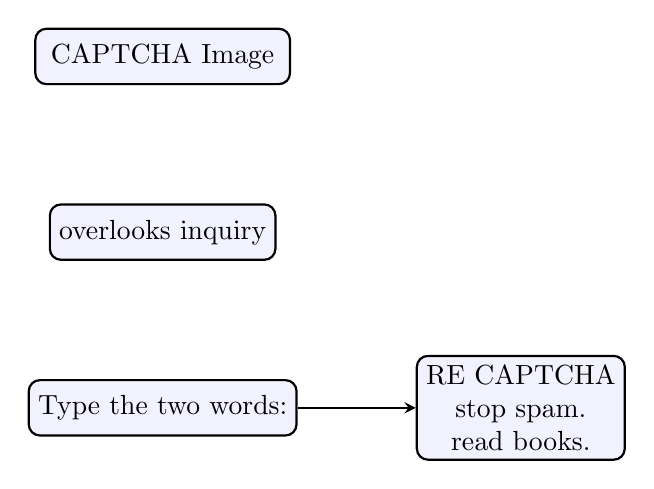
\begin{tikzpicture}[node distance=1.5cm, auto]
            \node[block, text width=3cm, align=center] (captcha) {CAPTCHA Image};
            \node[block, below=of captcha] (words) {overlooks inquiry};
            \node[block, below=of words] (input) {Type the two words:};
            \node[block, right=of input] (reCaptcha) {RE CAPTCHA \\ stop spam. \\ read books.};
            \draw[arrow] (input) -- (reCaptcha);
        \end{tikzpicture}
    \end{adjustbox}
    \caption{CAPTCHA Example}
    \label{fig:captcha}
\end{figure}

To further deter brute-force attacks, implement **CAPTCHAs** (Completely Automated Public Turing test to tell Computers and Humans Apart) or similar challenges to verify that the user is a human and not an automated bot (see Figure \ref{fig:captcha}).

\subsection{Weak Forgot-Password Processes}

A poorly designed **forgot-password process** can create significant security vulnerabilities.  Never email the user their actual password, as email is often transmitted in clear text and can be intercepted.  Similarly, avoid revealing whether an email address or username exists in the system.  Providing this information to an attacker allows them to narrow down their target list and launch more focused attacks.

Instead, always respond with a generic message indicating that password reset instructions will be emailed if the email address or username is valid.  When a user requests a password reset, send them a link (URL) containing a random, unique code associated with their account.  This link should expire after a short period.  Additionally, consider requiring users to enter a code sent to their registered phone number or email address as an extra verification step.

\subsection{Secure Password Storage}

Storing passwords in **plain text** or even in easily **encrypted** formats is a severe security risk. If the database is compromised, all passwords are immediately exposed.  The correct approach is to **always hash passwords with a random salt**.  The salt is a unique, randomly generated string added to each password before hashing. This prevents attackers from using precomputed tables of password hashes (rainbow tables) and makes it much more difficult to crack passwords even if the hash is stolen.

\subsection{Session Management}

**Session management** is the process of maintaining user state across multiple requests. Once a user has successfully logged in, the system needs to ensure that they have access to the appropriate resources on each subsequent page they visit. This is typically achieved using **session cookies** or similar mechanisms.  

A critical vulnerability arises when session validation is not consistently enforced on every page. The Panera Bread breach (see \href{https://krebsonsecurity.com/2018/04/panerabread-com-leaks-millions-of-customer-records/}{KrebsOnSecurity}) serves as a stark example.  Panera Bread failed to validate users on every page, allowing attackers to manipulate session IDs in the URL to access other users' accounts.  This highlights the importance of robust session management practices and consistent validation of user access rights.


% --- START OF CHUNK 9 ---

\section{Panera Bread and Software Integrity}

\subsection{The Panera Bread Incident}

The case of Panera Bread serves as a stark reminder of the importance of robust software and data integrity practices. In 2018, KrebsOnSecurity reported a significant vulnerability in Panera Bread’s website and mobile app.  The vulnerability allowed anyone to access customer data, including names, addresses, birthdays, and even partial credit card numbers. This wasn't due to a sophisticated hack, but rather a failure to adequately protect sensitive data within the application itself.  The root cause was a lack of proper authorization checks, allowing unauthorized access to customer profiles.  The website was temporarily taken offline as illustrated in the slide, with a simple "We apologize for any inconvenience" message, highlighting the disruption caused by this security lapse. This incident underscores the critical need for developers to implement and maintain strong security measures throughout the software development lifecycle.

\subsection{A08: Software and Data Integrity Failures}

The Open Web Application Security Project (OWASP) has identified **Software and Data Integrity Failures** as a key security risk, formally adding it as category A08 in their 2021 Top Ten list. This category focuses on vulnerabilities arising from assumptions about the correctness of software and data without proper verification.  Essentially, it's about trusting that things are working as expected without actually *checking* that they are. This can manifest in several ways, including insufficient validation of data inputs, reliance on untrusted sources for code or libraries, and a lack of integrity checks during software updates.  The consequences of such failures can range from data breaches and system compromise to denial-of-service attacks and even physical harm.

\subsection{Understanding the Risks}

Software and data integrity failures are particularly prevalent in modern software development environments that rely heavily on **cloud servers**, **Content Delivery Networks (CDNs)**, and **CI/CD pipelines**.  CDNs, while improving performance, introduce a new attack surface as malicious code could be injected into the CDN and served to users. Similarly, CI/CD pipelines, if not secured properly, can be exploited to inject malicious code into the deployment process.  A growing concern is the widespread use of **auto-update functionality**. While convenient, these updates are often downloaded without sufficient integrity verification, meaning a compromised update server could deliver malicious code directly to users' systems.  This is a prime example of making assumptions – assuming the update source is trustworthy – without verifying the integrity of the downloaded code.

\subsection{Preventing Integrity Failures}

Several measures can be taken to mitigate the risk of software and data integrity failures.  One crucial step is the implementation of **digital signatures**.  By digitally signing software updates, developers can ensure that the update has not been tampered with and that it originates from a trusted source.  Another best practice is to manage your own internal repositories for third-party libraries, such as NPM or NuGet. This allows you to control the versions of libraries used in your projects and to verify their integrity before deployment.  Furthermore, after each deployment, it's essential to calculate a **hash** (e.g., SHA-256) of the files and folders and compare it to the expected hash value. This ensures that the deployed code matches the intended code.  This hash verification should be automated and run frequently, ideally at least once a day.

\subsection{Additional Preventative Measures}

Beyond the core practices of digital signatures and hash verification, several other measures can enhance software and data integrity.  Regular **security and code scans** can identify potential vulnerabilities and coding errors that could lead to integrity failures.  **Manual code reviews** by experienced developers can provide an additional layer of scrutiny, catching issues that automated tools might miss.  Finally, it's crucial to secure your **CI/CD pipelines** by avoiding the storage of passwords in the pipeline configuration and limiting access to authorized personnel only.  A compromised CI/CD pipeline can be a gateway for attackers to inject malicious code into your software.

\section{Security Monitoring and Logging}

\subsection{The Importance of A09}

The OWASP Top Ten category **A09: Security Monitoring and Logging Failures** has gained prominence, moving up from #10 to #9 in the 2021 list.  This reflects the increasing recognition of the critical role that effective monitoring and logging play in detecting and responding to security incidents.  Previously known as "Insufficient Logging and Monitoring," this category highlights the need for organizations to proactively monitor their systems for suspicious activity and to maintain detailed logs that can be used for forensic analysis.  This category primarily concerns itself with understanding **traffic patterns** and the overall **health of an application**.

\subsection{Logging Best Practices}

Effective logging involves capturing all relevant **traffic and activity** to a site.  However, it's not enough to simply enable logging; you must also ensure that you are logging *enough* information to be useful in the event of a security incident.  A common misconception is that disk space is a limiting factor, but in reality, **disk space is relatively cheap**.  Therefore, you should log as much data as possible, offloading it to a separate server for storage and analysis.  Critically, **never leave logs on the server** itself. If the server is compromised, the logs can be altered or deleted by an attacker, hindering your ability to investigate the incident.

\subsection{Questions to Consider}

When evaluating your logging practices, consider the following questions: What is the application logging by default? Is it sufficient for security monitoring? What additional information *should* you be logging to provide better visibility into potential threats? Conversely, what information should you *not* log, such as sensitive personal data? Are the logs stored locally, or are they being sent to a centralized logging server? Finally, are there any errors or warnings in the logs that require attention? Regularly reviewing your logs and answering these questions can help you identify gaps in your logging strategy and improve your overall security posture.

\subsection{What Not to Log}

It is paramount to avoid logging **Personally Identifiable Information (PII)**. This includes names, addresses, social security numbers, and other data that could be used to identify an individual.  Similarly, you should never log **credit card numbers**, **bank account numbers**, or other sensitive financial information.  **Tokens**, **security keys**, and **passwords** should also be excluded from logs. Logging such information not only violates privacy regulations but also creates a significant security risk if the logs are compromised.

\subsection{Types of Logging}

Different types of logging provide different levels of insight into application behavior. **Exception logs** record unexpected crashes or errors in the application code. **Audit logs** track every page view, event, and transaction, providing a detailed record of user activity. **Usage logs** capture how frequently pages are viewed and features are used, helping you understand user behavior and identify potential performance issues. Finally, **security logs** record login attempts (both successful and failed) and access denials, providing valuable information for detecting and investigating security breaches.


% --- START OF CHUNK 10 ---
\section{Logging Rules and Security Logging}

\subsection{Importance of Logging}

Effective **logging** is a cornerstone of any robust security strategy. It provides a detailed record of events occurring within a system, enabling security professionals to detect, investigate, and respond to security incidents.  Without comprehensive logs, it's akin to investigating a crime scene with no witnesses or evidence.  We begin by establishing fundamental logging rules.  First, it is crucial to log all **normal traffic**, specifically the successful execution of paths within the application. This baseline of normal activity is essential for identifying deviations that may indicate malicious behavior.  Equally important is logging **any errors** encountered by the system. Errors can reveal vulnerabilities or indicate ongoing attacks.  

\subsection{Log Management and Tools}

Simply generating logs is insufficient; they must be effectively managed. This requires a dedicated **log management tool**.  These tools provide capabilities for centralized collection, storage, analysis, and alerting.  A popular and powerful option is **Splunk**, which offers advanced search, visualization, and reporting features.  Other options include the ELK stack (Elasticsearch, Logstash, Kibana) and Graylog. The choice of tool depends on the specific needs and resources of the organization.

\subsection{Specific Logging Requirements}

Beyond general traffic and errors, security logging requires a more focused approach.  All **logins** – both successful and failed – must be meticulously recorded. Failed login attempts are particularly valuable as they can indicate brute-force attacks or compromised credentials.  Furthermore, **all warnings and errors** should be logged, regardless of their apparent severity.  A seemingly minor warning could be a precursor to a more significant issue. Finally, it is vital to log **abnormal traffic** patterns. This includes unusual requests, unexpected data volumes, or access from unfamiliar locations.

\section{Monitoring and Prevention}

\subsection{The Value of Log Review}

**Logging is WORTHLESS** unless the logs are actively reviewed.  Logs are not a passive record; they are a dynamic source of intelligence.  Regular review allows security teams to identify anomalies, detect potential attacks, and gain insights into system behavior.  Specifically, any errors identified in the system must be reviewed and reported to the development teams **daily**. This rapid feedback loop is essential for addressing vulnerabilities and improving system security.  Moreover, a system should be in place to **alert** on specific thresholds or when certain types of traffic occur.  For example, an alert could be triggered if the number of failed login attempts exceeds a predefined limit.

\subsection{Preventative Measures}

Proactive prevention is key to minimizing the risk of security breaches. Several measures can be implemented to enhance logging and security.  First, ensure that all **login, access control, and server-side input validation failures** are logged and flagged as potential hack attempts.  These failures often indicate malicious activity.  Second, ensure that logs are generated in a format that is easily **consumed by logging tools**.  Standard formats like JSON or CEF are preferred.  Third, make sure logs are **encoded correctly** to prevent vulnerabilities such as **SQL Injection** or **Cross-Site Scripting (XSS)**.  Improperly encoded logs can be exploited by attackers to inject malicious code.

\subsection{Advanced Prevention Techniques}

Further preventative measures include ensuring that **high-value transactions** have a detailed **audit trail** with **integrity controls** to prevent tampering or detection.  This can be achieved using append-only database tables or **blockchain** technology.  Additionally, **alerting for suspicious activity** should be established, and **reports/dashboards** should be visible to the entire security team.  Transparency and collaboration are crucial for effective security.  Finally, a comprehensive **incident response and recovery plan** should be created, outlining the steps to be taken in the event of a security breach.  This plan should include procedures for containment, eradication, and recovery.

\section{Server-Side Request Forgery (SSRF)}

\subsection{Introduction to SSRF}

**A10: Server-Side Request Forgery (SSRF)** is a vulnerability that has recently re-emerged as a significant threat. It was previously on the OWASP Top 10 list but dropped off in 2017, only to return as a critical concern.  SSRF occurs whenever a web application is **fetching a remote resource without validating the user-supplied URL**. This allows an attacker to manipulate the server into making requests to unintended locations, potentially accessing sensitive data or performing unauthorized actions.

\subsection{How SSRF Works}

\begin{figure}[H]
    \centering
    \begin{adjustbox}{max width=\textwidth}
        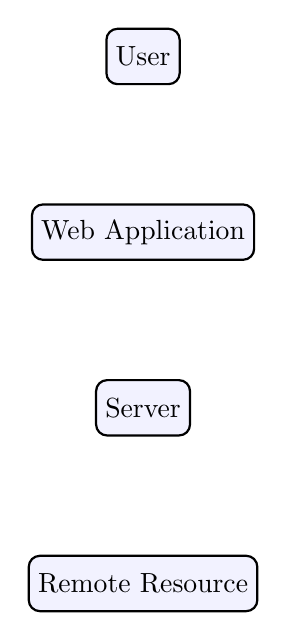
\begin{tikzpicture}[node distance=1.5cm, auto]
            \node[block, align=center] (user) {User};
            \node[block, below=of user] (app) {Web Application};
            \node[block, below=of app] (server) {Server};
            \node[block, below=of server] (remote) {Remote Resource};

            \path[arrow] (user) -- (app);
            \path[arrow] (app) -- (server);
            \path[arrow] (server) -- (remote);
        \end{tikzpicture}
    \end{adjustbox}
    \caption{SSRF Attack Flow}
\end{figure}

An attacker can exploit SSRF by crafting a malicious URL that causes the server to make a request to an internal resource or an external service. For example, consider a URL like \texttt{https://site.com/users/1234}. If the application does not validate the `1234` parameter, an attacker could change it to access different user accounts, as demonstrated in the **Panera Bread Hack**.

\subsection{Preventing SSRF}

The primary defense against SSRF is **input validation**.  The application must rigorously validate any user-supplied URLs before making requests to remote resources. This includes checking the URL's scheme, hostname, and path.  Additionally, consider using a **whitelist** of allowed URLs or domains.  By implementing these preventative measures, you can significantly reduce the risk of SSRF attacks.


\end{document}